\documentclass{beamer}
%\usepackage[latin1]{inputenc}
\usetheme{Warsaw}
\title[Intro to Python: Week 1]{Introduction  to Python\\ General Introduction, Basic Data Types, Functions}
\author{Christopher Barker}
\institute{UW Continuing Education / Isilon}
\date{June 20, 2012}

\usepackage{listings}
\usepackage{hyperref}

\begin{document}

\begin{frame}
\titlepage
\end{frame}

\begin{frame}
\frametitle{Table of Contents}
%\tableofcontents[currentsection]
\tableofcontents
\end{frame}

\section{Intro to the Class}

\begin{frame}{Instuctors}

Christopher Barker: \url{PythonCHB@gmail.com}

\vspace{0.5 in}

Dan Rutz: \url{danrutz@hotmail.com}

\end{frame}


\begin{frame}{Chris' History}

{\Large First computer:}
\begin{itemize}
  \item Commodore Pet -- 8k RAM
  \begin{itemize}
    \item  Basic
  \end{itemize}
\end{itemize}


{\Large High School:}
\begin{itemize}
  \item PDP 11 -- paper printer terminal 200baud modem 
  \begin{itemize}
    \item  Basic
  \end{itemize}
\end{itemize}

\pause

{\Large College: }
\begin{itemize}
  \item Pascal:  VAX/VMS  750 
  \item Scheme:  Unix VAX 780
\end{itemize}

\vspace{0.25in}

\pause

Then a long Break: Theater Arts Major, Scenery, Lighting...

\end{frame}

      

\begin{frame}{Chris' History}

    {\Large Back to School: PhD Engineering }
    \begin{itemize}
      \item     DOS / Windows 3.1
      \begin{itemize}
        \item  FORTRAN
        \item  MATLAB
        \item   Discovered Linux (RedHat 2.0)
      \end{itemize}
    \end{itemize}

   \vspace{0.25in}
     
    \pause 
    {\Large Now: }
    \begin{itemize}
       \item Oceanographer for NOAA
       \item Oil Spill Modeling
       \item Software Development
    \end{itemize}

    \pause 
    \vspace{0.25in}
    {\Large Gave TCL a try............ }
    
    \pause 
    \vspace{0.25in}
    {\Large Gave Perl a try............}

\end{frame}

\begin{frame}{Chris' History}
    
{\Large Discovered Python in 1998}
\begin{itemize}
    \item It could do what Perl could do,
    \begin{itemize}
        \item what TCL could do, what MATLAB could do,
    \end{itemize}
    \item But I liked it -- it fit my brain
\end{itemize}

\vspace{0.1in}

{\Large     My Python use now:}
\begin{itemize}
   \item Lots of text file crunching
   \item Lots of data processing scripts 
   \item Automation of downloading, processing data
   \item Desktop GUIs (wxPython)
   \item computational code
   \item wrapping C/C++ code      
   \item web apps (Pylons, Pyramid)
   \item GIS processing
   \item Ask me about "BILS" 
\end{itemize}
\end{frame}


\begin{frame}{Who are you?}

{\Large A bit about you:}
\begin{itemize}
  \item name
  \item What do you do at Islion?
  \item programing background (languages)
\end{itemize}

\end{frame}


\begin{frame}[fragile]{Class Structure}

{\LARGE github project} \\
\url{https://github.com/PythonCHB/PythonIntroClass}

\vspace{0.2in}
{\large Syllabus:} \\
\url{github.com/PythonCHB/PythonIntroClass/wiki/Syllabus} 

\vspace{0.2in}
{\large Code, etc:}

git: \\
\verb+https://github.com/PythonCHB/PythonIntroClass.git+

svn: \\
\verb+svn co https://github.com/PythonCHB/PythonIntroClass+

\end{frame}

\begin{frame}{Class Structure}

{\Large Class Time}
  \begin{itemize}
     \item Some lecture
     \item Lots of demos
     \item Lots of hand-on practice
     \item Interrupt me with questions -- please!
  \end{itemize}

\vspace{0.25in}
{\Large Homework}
  \begin{itemize}
     \item Assigned at each class
     \item Due Sunday night
     \item I'll review at the next class
  \end{itemize}


\end{frame}

\begin{frame}{Lightning Talks}

{\Large Lightning talks}
\begin{itemize}
   \item 5 minutes (including setup) - no kidding!
   \item Every student will give one
   \item Purposes: introduce yourself, share interests, also show Python applications
   \item Any topic you like, that is related to Python -- according to you!
\end{itemize}
\end{frame}


\section{What is Python?}

\begin{frame}{What is Python?}
    \begin{itemize}
      \item Dynamic
      \item Object oriented
      \item Byte-compiled
      \item interpreted
      \item ....
    \end{itemize}
\end{frame}

\begin{frame}{Python Ecosystem}

{\Large Used for:} 
\begin{itemize}
  \item CS education (this course!)  
  \item Application scripting (GIS, GNU Radio, Blender...)
  \item Systems administration and "glue"
  \item Web applications (Django etc. etc. etc.)
  \item Scientific/technical computing (a la MATLAB, Mathematica, also BioPython etc. ..)
  \item Software tools (automated software testing, distributed version control, ...)
  \item Research (natural language, graph theory, distributed computing, ...)
\end{itemize}

 An unusually large number of niches -- versatile
\end{frame}

\begin{frame}{Python Ecosystem}

{\Large Used by:} 
\begin{itemize}
  \item Beginners
  \item Professional software developers, computer system administrators, ...  
  \item Professionals OTHER THAN computer specialists: biologists, urban planners, ....
\end{itemize}
\vspace{0.25in}
 An unusually large number of types of users -- versatile\\[0.25in]
 You can be productive in Python WITHOUT full-time immersion!
\end{frame}


\begin{frame}{Python Features}
 
{\Large Gets many things right:}
\begin{itemize}
  \item  Readable -- looks nice, makes sense
  \item  No ideology about best way to program -- 
   object-oriented programming,  functional, etc.
  \item  No platform preference -- Windows, Mac, Linux, ...
  \item  Easy to connect to other languages -- C, Fortran - essential for science/math
  \item  Large standard library 
  \item  Even larger network of external packages
  \item  Countless conveniences, large and small, make it pleasant to work with
\end{itemize}
\end{frame}

\begin{frame}{Python Features}

{\Large Features:}

\begin{itemize}
  \item  Unlike C, C++, C\#, Java ... More like Ruby, Lisp, Perl, Matlab, Mathematica ...
  \item  Dynamic - no type declarations
    \begin{itemize}
      \item programs are shorter
      \item programs are more flexible
      \item less code means fewer bugs
    \end{itemize}
  \item  Interpreted - no separate compile, build steps - programming process is simpler
\end{itemize}

\end{frame}

\begin{frame}{Python Versions}

{\Large Python 2.*}

``Classic'' Python -- evolved from original

\vspace{0.25in}
{\Large Python 3.* (``py3k'')}

Updated version -- removed the "warts" allowed to break code (but really not all that different).
Not all that well adopted yet -- many packages not supported.

\vspace{0.25in}
This class uses Python 2.7 not Python 3

\end{frame}


\begin{frame}{Implementations}

\begin{itemize}
    \item Jython (JVM)
    \item Iron Python (.NET)
    \item PyPy -- Python written in Python (actually RPy...)
\end{itemize}

\vspace{0.25in}
  We will use CPython 2.7 from python.org for this course.

\end{frame}


\begin{frame}{A Tiny Bit of History}

Invented/developed by Guido van Rossum in 1989 -- first version was written on
a Mac. Time of origin similar to TCL and Perl.

   \begin{columns}[t] % contents are top vertically aligned
     \begin{column}[T]{4.5cm} % each column can also be its own environment
        \begin{tabular}[pos]{lr}
             Date   	&  Version \\
            \hline
            Dec 1989   	& started \\
            Feb 1991        &	0.9.0 \\
            Jan 1994         &    1.0.0 \\
            Apr 1999		  &   1.5.2 \\	
            Sept 2006	  &   2.5 \\
            Dec 2008	  &   	3.0 \\
            Jul 2010            	  &    2.7 \\
        \end{tabular}
     \end{column}
     \begin{column}[T]{5.5cm} % alternative top-align that's better for graphics
          GvR at Google -- still the BDFL \\
          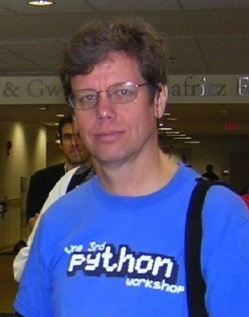
\includegraphics[height=2.0in]{GvR.jpg}
     \end{column}
   \end{columns}
Code swarm for Python history: \url{http://vimeo.com/1093745}

\end{frame} 


\begin{frame}[fragile]{What's a Dynamic language}

Strong, Dynamic typing.

 - Type checking and dispatch happen at run-time

\vspace{0.25in}
{\Large \verb!X = A+B!}
\vspace{0.1in}
\begin{itemize}
\pause
  \item What is A?
  \item What is B?
  \item What does is mean to add them?
\vspace{0.2in}
\pause
  \item A and B can change at any time before this process
\end{itemize}

\end{frame} 

\begin{frame}[fragile]{Using Python}

All you need for Python:
\begin{itemize}
  \item  A good programmer's text editor
    \begin{itemize}
      \item Good Python mode
      \item Particularly indentation!
    \end{itemize}
  \item  The command line to run code
  \item  The interactive shell
    \begin{itemize}
      \item regular interpreter
      \item \verb+IPython+ is an excellent enhancement\\
        \url{http://ipython.org/}
    \end{itemize}
\end{itemize}

\vspace{.2in}
There are lots of Editors, IDES, etc.:\\
   maybe you'll find one you like.

\end{frame} 

\begin{frame}[fragile]{Running Python Code}

\begin{itemize}
  \item At an interpreter prompt:\\
   \begin{verbatim}
     $ python 
     >>> print 'Hello, world!' 
     Hello, world!
   \end{verbatim}
\end{itemize}

\end{frame} 

\begin{frame}[fragile]{Running Python Modules}


{\Large Running Modules}\\[0.05in]
-- a file that contains Python code, filename ends with \verb+.py+

 \begin{enumerate}
    \item \verb+$ python hello.py+  -- must be in current working directory

    \item \verb+$ python -m hello+  -- any module on PYTHONPATH anywhere on the system

    \item \verb+$ ./hello.py+       -- put \verb+\#!/usr/env/python+ at top of module (Unix)
   
    \item \verb+$ python -i hello.py+  -- import module, remain in interactive session 

    \item \verb+>>> import hello+    -- at the python prompt -- importing a module executes its contents

    \item \verb+In [79]: run hello.py+    -- at the IPython prompt -- running a module brings the names into the interactive namespace
\end{enumerate}

\end{frame} 

\begin{frame}[fragile]{Documentation}

{\Large python.org docs:}

\url{http://docs.python.org/index.html}

\vspace{0.25in}
{\Large Particularly the library reference:}

\url{http://docs.python.org/library/index.html}

\vspace{0.25in}
(The tutorial is pretty good, too)

\end{frame} 

\begin{frame}[fragile]{PEPs}

{\large \url{http://www.python.org/dev/peps/} }

\vspace{0.25in}
\begin{description}
  \item[PEP 1]   PEP Purpose and Guidelines
  \item[PEP 8]   Style Guide for Python Code
  \item[PEP 20]  the Zen of Python
\end{description}

\end{frame} 

\begin{frame}[fragile]{pydoc}

Suite of tools for processing ``docstrings''

And an online source at the interpreter:

\begin{verbatim}
>>> from pydoc import help
>>> help(int)
Help on class int in module __builtin__:

class int(object)
 |  int(x[, base]) -> integer
 |  
 |  Convert a string or number to an integer, if possible.  A floating point
 ...
\end{verbatim}
or: \verb+$ pydoc+

(but I prefer IPython's  \verb+?+)

\end{frame} 

\begin{frame}[fragile]{Documentation}

{\LARGEgoogle}

\vspace{0.25in}
But  be careful!

\vspace{0.25in}
Lots of great info out there!

\vspace{0.25in}
Most of it is opinionated and out of date.\\
(might still be correct, though!)

\end{frame} 

\begin{frame}[fragile]{Lab}

{\Large Getting everyone on-line and at a command line.}

\begin{itemize}
    \item Log in
    \item Do a git or SVN checkout of the project
    \item Start up the Python interpreter:\\
          \verb+$ python+  ( \verb=ctrl+D= to exit )
    \item Run \verb+hello.py+
    \item Create a file in your editor and save it
    \item Start up \verb+IPython+ \\
          \verb+$ ipython+ ( also \verb=ctrl+D= to exit )
    \item Run \verb+hello.py+ in \verb+IPython+
    \item use \verb+?+ in \verb+IPython+ on anything...

if you have time:
\vspace{0.2in}
\url{http://learnpythonthehardway.org/book/ex1.html}
\url{http://learnpythonthehardway.org/book/ex2.html}

    
\end{itemize}

\end{frame} 


\section{Values, Expressions, and Types}


\begin{frame}[fragile]{Values, expressions, and types}

Values (data) vs. variables (names with values)

\begin{itemize}
    \item  Values are pieces of unnamed data: \verb+42, 'Hello, world',+

    \item  In Python, all values are objects\\
      Try \verb+dir(42)+ - lots going on behind the curtain! (demo)

    \item  Every value belongs to a type: integer, float, str, ...  (demo)

    \item  An expression is made up of values and operators, is evaluated to
        produce a value -- \verb+2 + 2+, etc.

    \item  Python interpreter can be used as a calculator to evaluate expressions (demo)

    \item  Integer vs. float arithmetic (demo)

    \item  Type errors - checked at run time only (demo)
  
    \item  Type conversions (demo)
\end{itemize}

\end{frame}

\begin{frame}[fragile]{Variables}

{\large Variables are names for values - objects}\\[0.1in]
\hspace{0.5in} - Variables don’t have a type; values do -- 
this is where the dynamic comes from

\begin{verbatim}
>>> type(42)
<type 'int'>
>>> type(3.14)
<type 'float'>
>>> a = 42
>>> b = 3.14
>>> type(a)
<type 'int'>
>>> a = b
>>> type(a)
<type 'float'>
\end{verbatim}

\end{frame}

\begin{frame}[fragile]{Assignment}

{\large Assignment is really name binding: }

Attaching a name to a value

A value can have many names (or none!)

\vspace{0.2in}
\verb+=+ assigns

\vspace{0.2in}
\verb+==+ checks equality

\vspace{0.2in}
\verb+is+ checks identity

\vspace{0.2in}
\verb+id()+ queries identity

\vspace{0.2in}
(demo)

\end{frame}

\begin{frame}[fragile]{Assignment}

{\Large  Multiple Assignment

\vspace{0.25in}

\verb+a, b = 1, 2+
}

\end{frame}


\begin{frame}[fragile]{Operator Precedence}

Operators Precedence determines what evaluates first:

\verb^4+3*5 != (4+3)*5^  --  Use parentheses !

Precedence of common operators:

Arithmetic \\
\verb!**! \\
\verb!+x, -x! \\	
\verb!*, /, %!	\\
\verb!+, -! \\

Comparisons:

\verb^<, <=, >, >=, !=, ==^

Boolean operators:
 
\verb!or, and, not!

Membership and Identity:

\verb!in, not in, is, is not!

\end{frame}



\begin{frame}[fragile]{string literals}

\begin{verbatim}
'a string'
"also a string"
"a string with an apostophe: isn't it cool?"
' a string with an embedded "quote" '
""" a multi-line
string
all in one
"""
"a string with an \n escaped character"

r'a "raw" string the \n comes through as a \n'
 
\end{verbatim}

\end{frame}

\begin{frame}[fragile]{key words}

{\Large  A bunch:}

\vspace{0.2in}
\begin{verbatim}
and       del       from      not       while    
as        elif      global    or        with     
assert    else      if        pass      yield    
break     except    import    print              
class     exec      in        raise              
continue  finally   is        return             
def       for       lambda    try
\end{verbatim}

\end{frame}

\begin{frame}[fragile]{and the built-ins..}

{\Large  Try this: 

\vspace{0.2in}
\verb+>>> dir(__builtins__)+

}
\end{frame}


\begin{frame}[fragile]{Lab}

{\large From LPTHW }

\vspace{0.2in}
\url{http://learnpythonthehardway.org/book/ex3.html}

\vspace{0.2in}
\url{http://learnpythonthehardway.org/book/ex4.html}

\vspace{0.2in}
\url{http://learnpythonthehardway.org/book/ex5.html}

(and 6 -- 8 if you get bored...)

\end{frame}

\section{Functions}


\begin{frame}[fragile]{Functions}

{\Large Minimal Function}

\begin{verbatim}
def <name>():
    <statement>
\end{verbatim}

\pause
{\Large Pass Statement (Note the indentation!)}
\begin{verbatim}
def <name>():
    pass
\end{verbatim}


\end{frame}

\begin{frame}[fragile]{Functions: def}

{\large \verb+def+ is a statement:}
\begin{itemize}
  \item it is executed
  \item it creates a local variable
\end{itemize}

\vspace{0.2in}{\largefunction defs must be executed before the functions can be called}

\pause
\vspace{0.2in}{\largefunctions call functions -- this makes a stack -- that's all a trace back is}

\end{frame}

\begin{frame}[fragile]{Functions: Call Stack}

\begin{verbatim}
def exceptional():
    print "I am exceptional!"
    print 1/0
def passive():
    pass
def doer():
    passive()
    exceptional()
\end{verbatim}

\end{frame}

\begin{frame}[fragile]{Functions: Tracebacks}

\begin{verbatim}
I am exceptional!
Traceback (most recent call last):
  File "functions.py", line 15, in <module>
    doer()
  File "functions.py", line 12, in doer
    exceptional()
  File "functions.py", line 5, in exceptional
    print 1/0
ZeroDivisionError: integer division or modulo by zero
\end{verbatim}

\end{frame}

\begin{frame}[fragile]{Functions: return}

{\Large Every function ends with a \verb+return+}

\begin{verbatim}
def five():
    return 5
\end{verbatim}

{\Large Actual simplest function}
\begin{verbatim}
def fun():
    return None
\end{verbatim}
\end{frame}

\begin{frame}[fragile]{Functions: return}

{\Large if you don't put \verb+return+ there, python will:}

\begin{verbatim}
In [123]: def fun():
   .....:     pass
In [124]: result = fun()
In [125]: print result
None
\end{verbatim}

{\Large note that the interpreter eats \verb+None+}

\end{frame}


\begin{frame}{Functions: return}

\vspace{0.25in}
{\Large Only one return statement will ever be executed.}

\pause
\vspace{0.25in}
{\Large Ever.}

\pause
\vspace{0.25in}
{\Large Anything after a executed return statement will never get run.}

\vspace{0.25in}
{\Large This is useful when debugging! }

\end{frame}


\begin{frame}[fragile]{Functions: return}

{\Large functions can return multiple results}

\begin{verbatim}
def fun():
    return 1,2,3

In [149]: fun()
Out[149]: (1, 2, 3)
\end{verbatim}

\end{frame}

\begin{frame}[fragile]{Functions: return}

{\Large remember multiple assignment?}

\begin{verbatim}
In [150]: x,y,z = fun()

In [151]: x
Out[151]: 1

In [152]: y
Out[152]: 2

In [153]: z
Out[153]: 3
\end{verbatim}

\end{frame}

\begin{frame}[fragile]{Functions: return}

{\Large Actually a tuple of results...}

\begin{verbatim}
In [154]: t = fun()

In [155]: t
Out[155]: (1, 2, 3)

In [156]: type(t)
Out[156]: tuple
\end{verbatim}

{\Large Multiple assignment is really "tuple unpacking"}

\end{frame}



\begin{frame}[fragile]{Functions: parameters}

{\Large function parameters: in definition}

\begin{verbatim}
def fun(x, y, z):
     q = x + y + z
     print x, y, z, q
\end{verbatim}

{\Large x, y, z are local names -- so is q}

\end{frame}

\begin{frame}[fragile]{Functions: arguments}

{\Large function arguments: when calling}

\begin{verbatim}
def fun(x, y, z):
     print x, y, z
\end{verbatim}
\begin{verbatim}
In [138]: fun(3, 4, 5)

3 4 5
\end{verbatim}

\end{frame}


\begin{frame}[fragile]{Functions: local vs. global}

\begin{verbatim}
x = 32
y = 33
z = 34
def fun(y, z):
     print x, y, z
\end{verbatim}
\begin{verbatim}
In [141]: fun(3,4)

32 3 4
\end{verbatim}
{\Large x is global, y, z are local}

\end{frame}

\begin{frame}[fragile]{Functions: local vs. global}

\begin{verbatim}
x = 3
def f():
    y = x
    x = 5
    print x
    print y
\end{verbatim}
  
{\Large What happens when we call \verb+f()+?}

\end{frame}

\begin{frame}[fragile]{Functions: local vs. global}

{\Large Gotcha!}

\begin{verbatim}
In [134]: f()
---------------------------------------------------------------------------
UnboundLocalError                         Traceback (most recent call last)
/Users/Chris/<ipython-input-132-9225fa53a20a> in f()
      1 def f():
----> 2     y = x
      3     x = 5
      4     print x
      5     print y
\end{verbatim}
  
{\Large you are going to assign x -- so it's local}

\end{frame}

\begin{frame}[fragile]{Scopes}

\vspace{0.5in}
{\LargeThere is a \verb+global+ statement}

\pause
\vspace{0.5in}
{\LARGE Don't use it!}

\end{frame}

\begin{frame}[fragile]{Scopes}

\vspace{0.5in}
{\Largegood discussion of scopes:}

\vspace{0.5in}
\url{http://docs.python.org/tutorial/classes.html#python-­‐scopes-­‐and-­‐namespaces}

\end{frame}

\begin{frame}[fragile]{Recursion}

\vspace{0.5in}
{\LargeRecursion is calling a function from itself.}

\vspace{0.5in}
{\LargeMax stack depth, function call overhead.}

\vspace{0.5in}
{\LargeBecause of these two(?), recursion isn't used {\bf that} often in Python.}

\end{frame}

\begin{frame}[fragile]{Lab: functions}

{\Large write a function that:}
\begin{itemize}
  \item takes a number and returns the square and cube of that number
   -- use local variables to store the results
  \item takes a string and a number, and returns a new string with the value repeated the given number of times
  \item uses both global and local variable to compute a result.
  \item calls another function to do part of its job.
  \item take some code with functions, add this to each function:
    \begin{verbatim}
        print locals()
    \end{verbatim}
  \item computes the factorial with a recursive function (needs something we haven't covered yet..)
\end{itemize}

\end{frame}


\section{Wrap Up}

\begin{frame}{Lightning Talks}

\vspace{0.5in}
{\Large Assign times for lightning talks}

\vspace{0.5in}
\center{\Large Let's use Python for that!} 

\end{frame}


\begin{frame}[fragile]{Wrap Up}

{\LargeAssignment -- Due midnight, Sun, June 24.}

\vspace{0.15in}
Think Python: Chapters (1), 2, 3, 4, 5, 6, 7, 8

\vspace{0.15in}
Pick something you'd like to automate that Python may be able to do. Write out a description of the problem


\vspace{0.15in}
Coding is the only way to learn to code.\\
CodingBat exercises are a good way to build skills.
\begin{itemize}
  \item visit \url{http://codingbat.com}
  \item sign up for an account
  \item goto ‘prefs’ page
  \item Share To: \url{PythonCHB@gmailcom}
\end{itemize}

Do two exercises from CodingBat: Warmup-1 

\end{frame}


\end{document}

 
